%% BEGIN semsamp2.tex
% This is a sample document for seminar.sty, v0.93 (and maybe later).
%
% This file contains both landscape and portrait mode slides.
% Choose one of the following to print them out:
%  - If using PSTricks, try the semcolor style option.
%  - If using Rokicki's dvips, try the semrot style option.
%  - To print the landscape slides, put \landscapeonly in the preamble.
%    To print the portrait slides, include the portrait style option and
%    put \portraitonly in the preamble.
%
%
\documentclass[%
%rrrrrrrrrrrrrrrr\documentstyle[%
  slidesonly,%  Try notes or notesonly instead.
  %10pt,%notes,%      Use instead of slidesonly to typeset the notes.
  %notesonly,%  Use instead of slidesonly to typeset notes and slides.
  %semcolor,%   Try me if using PSTricks.
  %semrot,%     Try me if using Rokicki's dvips.
  %semhelv,%    Try me if using a PostScript printer.
  %article,%    Try me.
  %portrait,%   Try me.
  %sem-a4,%     Try me if using A4 paper.
  semlayer%     This must be included, but you need the semcolor option to
  ]{seminar}                                  % actually see the overlays.

\slidesmag{5}
\articlemag{1}

%\twoup                     % Try me for twoup printing.

%\portraitonly              % To print only portrait slides
%\landscapeonly             % To print only landscape slides

%\notslides{\ref{questions}-7,1}   %Try me: The slides are omitted.
%\onlyslides{\ref{questions}-7,1}  %Try me: Only these slides are included.
%\onlynotestoo                     %Try me: For selecting notes as well.

\colorlayers{red,blue}      % Try deleting this if using the semcolor option,
                            % to get \blue and \red to use PostScript color.

%\overlaysfalse             % Suppress overlays with semcolor option.
%\layersfalse               % Suppress color layers with semcolor option.

\rotateheaderstrue          % Try this out if using rotation macros.

\usepackage{hyperref}
\usepackage{url}
\usepackage{amsmath}
\usepackage{amsthm}
\usepackage{graphicx}
% \usepackage[pdftex]{graphicx}
\usepackage{amsfonts}
\usepackage{mathrsfs}
\usepackage{amssymb}
\usepackage[noend]{algorithmic}
\usepackage[plain]{algorithm}
\usepackage{subfigure}

\usepackage{color}
\usepackage{ulem}

%\newtheorem{theorem}{Theorem}[section]
\newtheorem{theorem}{Theorem}
\newtheorem{corollary}{Corollary}[section]
\newtheorem{lemma}{Lemma}[section]
\newtheorem{definition}{Definition}[section]
\newtheorem{proposition}{Proposition}[section]
\newtheorem{claim}{Claim}[section]
\newtheorem{model}{Model}[section]
\newtheorem{example}{Example}[section]
%\newtheorem{algorithm}{Algorithm}[section]
%\newenvironment{proof}{\noindent{\bf Proof.}}{\hspace*{\fill} $\Box$}
%\newenvironment{defn}{\noindent \underline{\hspace{7in}}\\ \noindent{\bf Defn:}}{\hspace*{\fill} \newline\noindent\underline{\hspace{7in}}}
\newenvironment{defn}{\noindent \\ \noindent{\bf Defn:}}{\hspace*{\fill} \newline}
\newcommand{\fns}{\footnotesize}
\newcommand{\sk}{\sf{sk}}
\newcommand{\pk}{\sf{pk}}
\newenvironment{thm}{\noindent{\bf Theorem:}}{\hspace*{\fill} }
\newcommand{\bare}{\noindent \underline{\hspace{7in}}\\ }
%\newcommand{\myws}{\textcolor{white}{ XXXXXX}}
\newcommand{\vt}{

\vspace{.15in} 

\noindent}

\newcommand{\nvt}{

\vspace{-.15in} 

\noindent}
%\newenvironment{thm}{\noindent{\bf Theorem:}}{\hspace*{\fill} }
%\newcommand{\bare}{\noindent \underline{\hspace{7in}}\\ }
%\newcommand{\myws}{\textcolor{white}{ XXXXXX}}
%\newcommand{\mybul}{{\textcolor{white}{XX}}$\bullet$ }
\newcommand{\myar}{\textcolor{red}{ ==$>$}}
\newcommand{\mybl}{{\textcolor{white}{XX}}{\bf *}}
\newcommand{\n}{\noindent }

\newcommand{\mylg}{\mbox{ lg } }



\newcommand{\tht}{\hspace{.15in} }

\newcommand{\Half}{\mbox{\bf Half}}
\newcommand{\Solve}{\mbox{\bf Solve}}
\newcommand{\Halfc}{\underline{\mbox{\bf Half}}}
\def\4halftbs{XXX\=XXXX\=XXXX\=mmm\kill}

\def\tbs{XXXXXXX\=XXXXX\= \kill}
\def\otbs{XXXXXXX\=XXXXX\=XXX\=XXX\= \kill}
\def\sqrotbs{xxx\=xxx\=xx\kill}
\def\lsqrotbs{xxx\=xxx\=xxx\=xxBBBBBBBBBBBBBBBBBBBBBBBBBBBB\=xxx\=lxx\=xx\kill}
\def\monttbs{xx\=xxxx\=xxxx\=xxxx\kill}
\def\knudtbs{xxx\=xxxx\=xxxx\=xxxx\kill}

\renewcommand{\baselinestretch}{1}
\setlength{\unitlength}{.1in}
\addtolength{\textheight}{1.3in}
\addtolength{\topmargin}{-1.3in}
\addtolength{\textwidth}{1.88in}
\addtolength{\evensidemargin}{-1in}
\addtolength{\oddsidemargin}{-.9in}

\title{Chapter 1: Introduction}
\author{}
\date{}

\newcommand{\sref}[1]{SLIDE \ref{#1}}
\newcommand{\heading}[1]{\begin{center}\large\bf #1\end{center}}

\newpagestyle{MH}%
  {Purdue School of Eng \& Tech Graduate Student \LaTeX Workshop\hfil\thepage}{}
\pagestyle{MH}



%\begin{document}
\def\otbs{XXXXXXX\=XXXXX\=XXX\=XXX\= \kill}
\def\proofpartbs{XXX\=XXXXXxxxxxxxxxxxxxxxxxxx\=XXX\=XXX \kill}
\date{}
\newcommand{\ovec}{\overline}
\newcommand{\ds}{\displaystyle}
\newcommand{\ar}{\longrightarrow}
\newcommand{\p}{\prime}
\newcommand{\z}{{\bf Z}}
%\newcommand{\r}{{\bf R}}
\newcommand{\ex}{\noindent {\bf Example} }
\newcommand{\ra}{{\ Longrightarrow}}
\newcommand{\md}{{\makebox{ mod }}}
%\newcommand{\n}{{\noindent}}
\newcommand{\deriv}{\ds{\frac{dy}{dx}}}
\newcommand{\recipderiv}{\ds{\frac{dx}{dy}}}
\newcommand{\tab}{{\hspace{.3in}}}
\def\monttbs{xx\=xxxx\=xxxx\=xxxx\kill}
%\newcommand{\tht}{\hspace{.15in} }
\newcommand{\myws}{\textcolor{white}{XX}}
\newcommand{\mybul}{{\textcolor{white}{XX}}$\bullet$ }
\newcommand{\mystr}{{\textcolor{white}{XXXXXX}}$ \diamondsuit $ }
%\newcommand{\myar}{\textcolor{red}{ ==$>$}}
\newcommand{\la}{\longleftarrow}
\newcommand{\ty}{\textcolor{red}}
% Math-mode symbol & verbatim
\def\W#1#2{$#1{#2}$ &\tt\string#1\string{#2\string}}
\def\X#1{$#1$ &\tt\string#1}
\def\Y#1{$\big#1$ &\tt\string#1}
\def\Z#1{\tt\string#1}




%\pagestyle{empty}
\newcommand{\nhp}{\mbox{\it No half point}}
%\def\tbs{xxx\=95 - 100 $\%$\=xxxx\=95 - 100 $\%$\=xxxx\=95 - 100 $\%$
%\=xxxx\=95 - 100 $\%$\=xxxx\=95 - 100 $\%$\=xxxx\=mmm\kill}
\def\mtbs{xxxxxxx\=95 - 100 $\%$\=xxxx\= xxxxx\=\kill}
\def\smtbs{xxxxxxx\=95 - 100 $\%$xxxxxxxxxxxxxxx\= xxxxx\kill}
\def\sqrotbs{xxx\=xxx\=xx\kill}
%\def\lsqrotbs{xxx\=xxx\=xxx\=xxBBBBBBBBBBBBBBBBBBBBBBBBBBBB\=xxx\=lxx\=xx\kill}
\def\pkcset{\= $|E_{a_2,a_6}|=p\cdot 2$xxxx \= cofactor $2$xxx \=  $|(x,y)|=2n$ bitsxxxx \= compressed to $n$\kill}


%\def\lsqrotbs{xxx\=xxx\=xxBBBBBBBBBBBBBBBBBBBBBBBBBBBB\=xxx\=lxx\=xx\kill}

%.b.b.b.b.\def\lsqrotbs{xxx\=xxx\=xxx\=xxBBBBBBBBBBBBBBBBBBBBBBBBBBBB\=xxx\=lxx\=xx\kill}
\def\lsqrotbs{xxx\=xxx\=xxx\=xxBBBBBBBBBBBBBBBBBBBBBBBBBBBB\=xxx\=xxx\=lxx\=xx\kill}


% *********************************************************************************
% *****************************************************************
\newcommand{\mfor}{{\bf for }}
\newcommand{\mdo}{{\bf do }}
\newcommand{\melse}{{\bf else }}

\newcommand{\mif}{{\bf if }}
\newcommand{\mthen}{{\bf then }}
\newcommand{\mwhile}{{\bf while }}
\newcommand{\htab}{\tab}

\newcommand{\vtab}{{

\vspace{.2in} 

\n}}
\begin{document}
\DeclareGraphicsExtensions{.pdf, .bmp,.png,.gif,.jpg}


\maketitle          % This won't show up when \onlynotestoo is in effect.

\begin{slide}
  \ifslidesonly              % Title slide only for slidesonly selection.
    %\maketitle
    \addtocounter{slide}{-1}
    \slidepagestyle{empty}
  \fi
\end{slide}


\begin{slide}

\footnotesize

\begin{center}
\section*{Secure Data Aggregation Protocol for Sensor Networks}
  \vfill
  Presented By : Kavit Shah

  Major Advisor : Brian King
  
  Thesis Committee Members : Paul Salama, Mohamed El-Sharkawy, Sangkook Lee
  \vfill
  \end{center}
  \clearpage

\section*{Overview}
  \vfill
  \begin{center}
    \begin{itemize}
      \item Introduction
      \item Cryptographic Tools
      \item Data Aggregation
      \item Secure Hierarchical In-network Data Aggregation (SHIA)
      \item Our Protocol
      \item Conclusion
    \end{itemize}
  \end{center}
  \vfill
  \clearpage

\section*{Introduction}
  \vfill
  \begin{description}
    \item[Ubiquitous Computing -] is a scenario in which computing is everywhere.

    \item[Internet of Things -] is a system where the Internet is connected to physical world via ubiquitous sensors.
    
    \item[Ad-hoc Networking -] is a local network of sensors formed by peer-to-peer communications.
    
    \item[Sensor Networks -] Collectively, we refer these concept as Sensor Networks.
  \end{description}
  \vfill
  \clearpage

  \subsection*{Sensor Networks}
    \vfill  
    In sensor networks, thousands of sensors may interact with each other and collects raw data.

    The data is processed by computationally powerful machine (the base station).

    Then the base station converts data into information.

    Based on the derived information an important action is taken.

    % \begin{figure}[h!]
    %   \centering
    %   % \includegraphics{images/swon.pdf}
    %   % 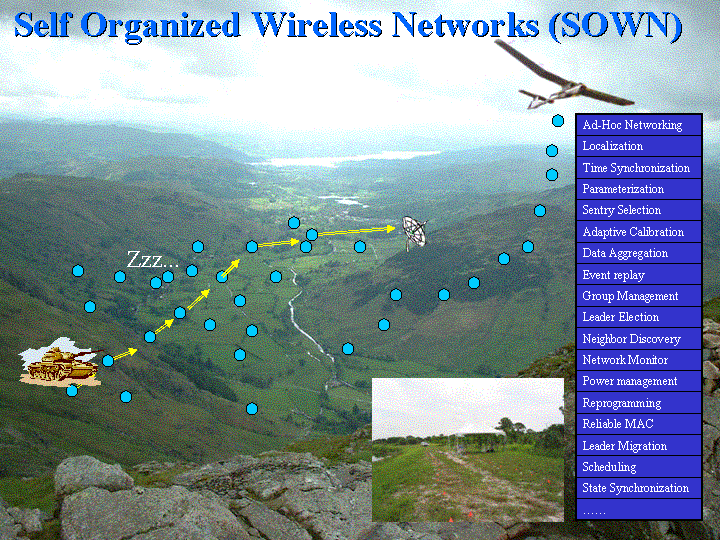
\includegraphics{swon.png}
    %   \caption{Sensor Network}
    %   \label{fig:sensor-network}
    % \end{figure}
    \vfill
    \clearpage

  \subsection*{Sensor Networks Applications}
    \vfill
    \begin{description}
    \item[Military -] enemy tracking, battle filed surveillance or target classification.

    \item[Environmental -] to monitor geographical location without much human intervention.
    
    \item[Health Care -]  to monitor patients around the clock, send reminders to doctors and nurses.
  
    \item[Sustainable Mobility -] to build digitally connected and coordinated vehicles.
    \end{description}
    \vfill
    \clearpage

  \subsection*{Consequences of Sensor Failures}
      \vfill
      Speed sensor failure led to crash of Air France flight - Airbus A330 on 1st June 2009.
      
      \textbf{For nearly a minute}, as the speed sensors jumped, the pilot was not present in the cockpit. 

      The pilots could not reclaim control as the plane dropped out of the sky at a rate of \textbf{10,000 feet per minute}.
          
      The flight plunged into the Atlantic nose-up after its three-and-a-half minute freefall , killing all \textbf{228} on board.      
      \vfill
      \clearpage

  \subsection*{Resource Constrains in Sensor Network}
    \vfill
    \begin{description}
      \item[Physical Limitations -] often deployed in open, hostile and unattended environments.

      \item[Hardware Limitations -] due to lower manufacturing cost of sensor nodes, they have low speed processor, limited storage, a short range trans receivers.

      \item[Transmission Medium -] wireless networks have approximately \textbf{$10^6$ times higher bit error rate (BER)} than wired networks which causes frequent link loss and then path loss.

      \item[Mobility -] network topology is dynamic, topology changes due to link failure, node failure or bandwidth optimization.
    \end{description}
    \vfill
    \clearpage

\section*{Cryptographic Tools}
  \vfill
  \subsection*{Hash Functions}
    A hash function takes a message as its input and outputs a fixed length message called hash code, creating a digital fingerprint of the message.

    % A hash function $h$ should have the following properties :
    \begin{description}
      \item [Compression] A function $h$ maps an input $x$ of arbitrary finite bitlength, to an output $h(x)$ of fixed bitlength $n$.
      \item [Preimage resistance] For all pre-specified outputs, it is computationally infeasible to find any input which hashes to that output, i.e., to find any preimage $x'$ such that $h(x') = y$ where $y$ is given whose corresponding input is not known.
      \item [2nd-preimage resistance] It is computationally infeasible to find any second input which has the same output as any specified input, i.e, given $x$, to find a 2nd-preimage $x' \neq x$ such that $h(x') = h(x)$.
      \item [Collision resistance] It is computationally to find any two distinct inputs $x,x'$ which hash to the same output, i.e., such that $h(x) = h(x')$.
    \end{description}
    SHA-256, is a 256-bit hash and provides $128$ bits of security against collision attacks.
    \vfill
    \clearpage

  \subsection*{Message Authentication Codes}
    \vfill
    A Message Authentication Code (MAC) is a family of hash functions parameterized by a secret key $k$.

    \begin{description}
      \item [Ease of computation] For a known function $h_{k}$, given a value $k$
      and an input $x$, $h_{k}(x)$ is easy to compute.
      \item [Compression] A function $h_{k}$ maps an input $x$ of arbitrary finite bitlength to an output $h_{k}(x)$ of fixed length $n$.  
      \item [Computation-resistance] Given a description of the function family $h$, for every fixed allowable value of $k$ (unknown to an adversary), given zero or more text-MAC pairs ($x_{i}, h_{k}(x_{i})$), it is computationally infeasible to compute any text-MAC pair ($x,h_{k}(x)$) for any new input $x \neq x^{'}$ (including possibly for $h_{k}(x) = h_{k}(x_{i})$ for some $i$). 
      If computation-resistance does not hold, a MAC algorithm is subject to MAC-forgery.
    \end{description}
    \vfill
    \clearpage

  \subsection*{Digital Signatures}
    \vfill
    A digital signature is a cryptographic scheme for demonstrating the authenticity of a digital message.
    
    A valid digital signature gives a recipient strong reason to believe that the message was created by a known sender, such that the sender can not deny having sent the message (\textbf{authentication and non-repudiation}) and that the message was not altered in transit (\textbf{integrity}).

    It is a 5-tuple scheme ($\mathcal{M}$, $\mathcal{K}$, $\mathcal{G}$, $\mathcal{S}$, $\mathcal{V}$)

    % \begin{enumerate}
    %   \item a plain text message space $\mathcal{M}$ (set of strings over alphabets)
    %   \item a signature space $\mathcal{S}$ (set of possible signatures)
    %   \item a signing key space $\mathcal{K}$ (set of possible keys for signature generation) and a verification space $\mathcal{K^{'}}$ (a set of possible verification keys)
    %   \item an efficient key generation algorithm \textsf{Gen} : $N \rightarrow$ $\mathcal{K} \times \mathcal{K^{'}} $ 
    %   \item an efficient signing algorithm \textsf{Sign} : $ \mathcal{M} \times \mathcal{K} \rightarrow \mathcal{S}$
    %   \item an efficient verification algorithm \textsf{Verify} : $\mathcal{S} \times \mathcal{M} \rightarrow$ \{true, false\} 
    % \end{enumerate}
    For any secret key $s_{k} \in \mathcal{K}$ and any $m \in \mathcal{M}$, the message $m$ is signed using key $s_{k}$ as follows:
      \begin{equation}
        s = \textsf{Sign}_{s_{k}}(m)
        \label{eq:signature}
      \end{equation}
    For any $s_{k}$ let $p_{k}$ denote public key and for all $m \in \mathcal{M}$ and $s \in \mathcal{S}$, $s$ as follows:
    \begin{equation}
      \textsf{Verify}_{p_{k}}(m,s) = 
      \begin{cases}
       \textbf{true}\ \mbox{with probability of 1} & \mbox{if}\ s = \textsf{Sign}_{s_{k}}(m)\\
       \textbf{false}\ \mbox{with overwhelming probability} & \mbox{if}\ s \neq \textsf{Sign}_{s_{k}}(m)
      \end{cases}
      \label{eq:verification}
    \end{equation}
    where the probability space is determine by the $\mathcal {M, S, K, K^{'}}$ and perhaps the signing and verification algorithms.
    The ``overwhelming probability'' for the signature scheme determines the probability that the scheme allows for a forgery.
    % The message is hashed before its being signed to reduce the message size. 
    % If the message is not hashed before signing then the signature can be longer than the message which is problematic for the longer messages.
    \vfill
    \clearpage

  \subsection*{Summary of Cryptography Tools}
    \vfill
    Three different integrity-protection mechanisms HASH, MAC, Signature are summarized here.
    \begin{table}[!htb]
      \tiny
      \begin{center}
        \begin{tabular}{ |l || l| l| }
          \hline
           & Who can generate it & Who can verify it \\
          \hline
          Hash & Everyone & Everyone \\ 
          \hline
          MAC & Holders of secret & Holders of secret \\
          \hline
          Signature & Holder of secret & Everyone \\
          \hline
        \end{tabular}
      \end{center}
    \end{table}
    \vfill
    \clearpage

\section*{Data Aggregation}
  \vfill
  The idea of Data Aggregation is to compress the data coming from different sources enroute eliminating redundancy, minimizing the number of transmissions, thus saving energy and increasing the longevity of the network.

  This paradigm shifts the focus from the traditional \textbf{address centric} approaches for networking (finding short routes between pairs of addressable end nodes) to a more \textbf{data-centric} approach (finding routes from multiple sources to a single destination that allows in-network consolidation of redundant data).
  \vfill
  \clearpage

  \subsection*{Definition}
      \vfill
      Consider a sensor network with $n$ sensors collecting data and the base station, processes data into information. 
      
      This can be represented as $f(x_{1}, x_{2},...,x_{n})$ where $x_{1}, x_{2},..., x_{n}$ represent the sensor readings.
      
      % Here $f$ is some mapping $f: \mathcal{D}_{1} \times \mathcal{D}_{2} \times ... \mathcal{D}_{n}$ $\rightarrow$ $I$, where $\mathcal{D}_{i}$ represents sensor $i$'s domain and $I$ represents the set of all possible information. 

      The goal is to compute the information as follows :
      \begin{equation*}
        y =\ f(x_{1}, x_{2},...,x_{n})
      \end{equation*}
      \vfill
      \clearpage

  \subsection*{Data Aggregation using SUM}
    \vfill      
    \begin{figure}
      \centering
      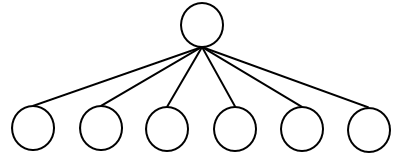
\includegraphics[scale = 0.4]{images/star-tree.png}
    \end{figure}

    The root in the network, receives the following sensor data $S_{1}(10), S_{2}(14), S_{3}(12), S_{4}(15), S_{5}(11),S_{6}(17)$ and has its own data $S_{0}(15)$. 

    The root node aggregates these seven data and creates an aggregated result as follows:
    \begin{equation}
      S = \sum_{i=0}^6 S_{i}
    \end{equation}
    Now, root has to send only one data to its parent instead of seven.
    \vfill
    \clearpage

  \subsection*{Lossy Data Compression}
    \vfill
    Lossy data compression schemes produces a compressed file from which only an \textbf{approximation} to the original information can be recovered. Much higher compression ratios are possible.

    Our aggregation protocol is \textbf{lossy data compression} as the base station receives an aggregated sensor data and can not recover the original sensor data.
    \vfill
    \clearpage

\section*{Secure Hierarchical In-network Data Aggregation}
    \vfill
    SHIA is a light weight protocol for providing data-integrity to in-network data aggregation scheme.
    
    It is designed for general networks with single or multiple adversaries.
    
    Our work enhances SHIA, by making it communication efficient, adds new security services to the protocol, achieves similar security goals with non-resilient aggregation functions and efficient ways of analyzing the protocol.
    \vfill
    \clearpage

    \subsection*{Network Assumptions}
      \vfill
      A multi hop network with a set $ S = \{S_{1},...,S_{n}\} $ of $n$ nodes where all sensor nodes are alive and reachable. 

      The network is organized in a \textbf{rooted tree topology}.

      The \textbf{trusted base station} resides outside of the network and the network and the network topology. 

      The base station can directly communicate with every node in the network using \textbf{authenticated broadcast}.

      All the wireless communications is \textbf{peer-to-peer} and we do not consider the \textbf{local wireless broadcast}.

      Each sensor node $I$ has a unique \textbf{ID} and shares a unique secret symmetric key $\sf{sk}_{I}$ with the base station.

      The sensor nodes are capable of doing \textbf{symmetric and asymmetric} key encryption and decryption.
      \vfill
      \clearpage

    \subsection*{Attacker Model}
      \vfill
      We consider a model with \textbf{polynomially bounded} adversary (polynomial in terms of the security parameter), which has a complete control over some of the sensor nodes in the network.
   
      We focus on \textbf{stealthy attacks}, where the goal of an adversary is to make the base station accept false aggregation  results, which are significantly different from the true results determined by the measured values, while not being detected by the base station.
      
      We do not consider \textbf{denial-of-service (DoS)} and various \textbf{passive attacks}.
      \vfill
      \clearpage

    \subsection*{SUM Aggregate Algorithm}
      \vfill
      Here, the aggregate function $f$\ is summation meaning that we want to compute $a_{1} + a_{2} + \dotsc + a_{n}$, where $a_{i}$\ is the sensor reading of the node $i$.
 
      The algorithm has the following three main phases.
      \begin{description}
        \item [Query Dissemination,] initiates the aggregation process.
        \item [Aggregate Commit,] initiates the commitment tree generation process.
        \item [Result Checking,] initiates the distributed, interactive verification process.
      \end{description}
      \vfill
      \clearpage

    \subsection*{Aggregation Tree}
      \vfill
      We require the prior constructed rooted aggregation tree.
      \begin{figure}[h!]
        \centering
        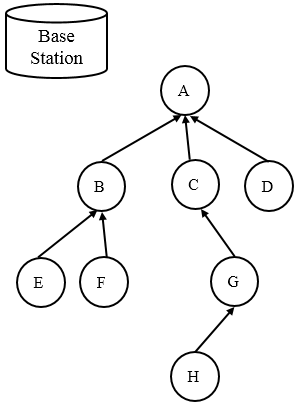
\includegraphics[scale=0.4]{images/aggregation-tree-1.png}
        \label{fig:Aggregation-tree-1}
        % \caption{c}
      \end{figure}
      \begin{center}
        Figure 1: Aggregation Tree
      \end{center}
      \vfill
      \clearpage

    \subsection*{Query Dissemination}
      \vfill
      The base station broadcasts the query request message with the query nonce $N$\ in the aggregation tree. 
    
      SHIA uses \textbf{hash chain} to generate new nonce for each query. 
      
      A hash chain is constructed by repeatedly evaluating a pre-image resistant hash function $h$\ on some initial random value, the final value (or ``anchor value'') is preloaded on the nodes in the network.
      
      The base station uses the pre-image of the last used value as the nonce for the next broadcast.
      
      \begin{figure}[h!]
        \centering
        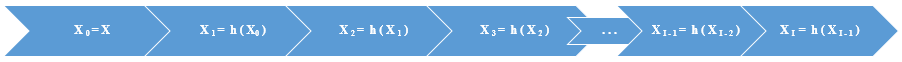
\includegraphics[scale=0.4]{images/hash-chain.png}
        \label{fig:hash-chain}
      \end{figure}
      \begin{center}
        Hash Chain.
      \end{center}

      For example, if the last known value of the hash chain is $h^i(X)$, then the next broadcast uses $h^{i-1}(X)$ as the nonce; $X$ is the initial random value.
      
      When a node receives a new nonce $N^{'}$, it verifies that $N^{'}$ is a precursor to the most recently received (and authenticated) nonce $N$ on the hash chain, i.e., $h^{i}(N^{'}) = N$ for some $i$ bounded by a fixed $k$ of number of hash applications.  
      \vfill
      % A hash chain prevents an adversary from predicting the query nonce for future queries as it has to reverse the hash chain computation to get an acceptable pre-image.
      \clearpage

    \subsection*{Aggregate Commit}
      \vfill
      \begin{defn}
        A commitment tree is a tree where each vertex has an associated label representing the data that is passed on to its parent: $<$count, value, complement, commitment$>$
      \end{defn}

      The sensor node $A$ creates the label for the leaf vertex $A_{0}$ is given as follows :
      \begin{tiny}
      \begin{equation*}
        A_{0} =\ <A_{count}, A_{value}, \overline{A_{value}}, A_{commitment}>
      \end{equation*}
      \end{tiny}
      Internal node $I$ has child vertices:
      \begin{tiny}
       $A_{1}$, $A_{2}$, $\dotsc$ , $A_{q}$; $A_{i}$ = $<$ $A_{icount}$, $A_{ivalue}$, $\overline{A_{ivalue}}$, $A_{icommitment}$$>$.
      \end{tiny}
      Then,
      \begin{tiny}
        \begin{equation*}
          \begin{array}{l}
            I_{j} =\ <I_{jcount}, I_{jvalue}, \overline{I_{jvalue}}, I_{jcommitment}>\\
            I_{jcount} = \sum A_{icount}\\ 
            I_{jvalue} = \sum A_{ivalue}\\
            \overline{I_{jvalue}} = \sum \overline{A_{ivalue}}\\
            I_{jcommitment} = H[N||I_{jcount}||I_{jvalue}||\overline{I_{jvalue}}||A_{1}||A_{2}|| \dotsc ||A_{q}]\\
          \end{array}
        \end{equation*}
      \end{tiny}
      
      \vfill
      \clearpage

    \subsection*{Commitment Tree Generation Algorithm}
      \vfill
      Leaf nodes in the aggregation tree originate a single-vertex commitment forest.

      Internal node $I$ originates a similar single-vertex commitment forest and receives commitment forests from its children.
      
      $I$ wishes to combine $q$ commitment forests $F_{1}$,$\dotsc$,$F_{q}$.
      
      The intermediate result be $F$ $=$ $F_{1}$ $\cup$ $\dotsc$ $\cup$ $F_{q}$, and repeat the following until no two trees are the same height in $F$.
      
      Let $h$ be the smallest height such that more than one tree in $F$ has height $h$.
      
      Find two commitment trees $T_{1}$ and $T_{2}$ of height $h$ in $F$, and merge them into a tree of height $h + 1$ by creating a new 
      vertex that is the parent of both the roots of $T_{1}$ and $T_{2}$.
      \vfill
      \clearpage
    \subsection*{Commitment Tree Generation Example}
      \vfill
      The commitment tree generation for the root $A$ of Figure 1 is given as follows:
      \begin{figure}
        \centering
        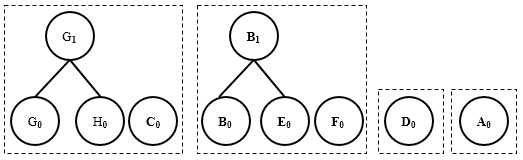
\includegraphics[scale = 0.4]{images/a-forest-shia.png}
      \end{figure}
      \begin{tiny}
      \begin{center}
        $A$'s forest impacted by the forests received from $B, C, D$.
      \end{center}
      \end{tiny}
      \begin{figure}
        \centering
        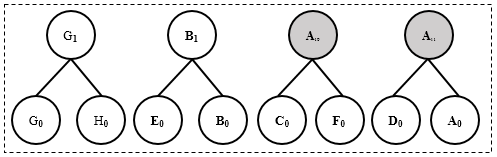
\includegraphics[scale = 0.4]{images/a-forest-first-merge-shia.png}
      \end{figure}
      \begin{tiny}
      \begin{center}
        $A$'s forest after first merge.
      \end{center}
      \end{tiny}
      \begin{figure}
        \centering
        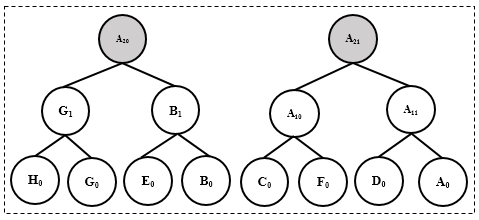
\includegraphics[scale = 0.4]{images/a-forest-second-merge-shia.png}
      \end{figure}
      \begin{tiny}
      \begin{center}
          $A$'s forest after second merge.
      \end{center}
      \end{tiny}
      \begin{figure}
        \centering
        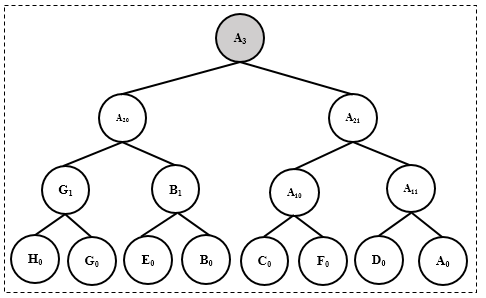
\includegraphics[scale = 0.4]{images/a-payload-shia.png}
      \end{figure}
      \begin{tiny}
        \begin{center}
            $A$'s outgoing forest.
        \end{center}
      \end{tiny}

      \begin{tiny}
      \begin{equation*}
        \begin{array}{l}
          A_{3} = <8, A_{3value}, \overline{A_{3value}}, H(N || 8 || A_{3value} || \overline{A_{3value}} || A_{20} ||A_{21}) >\\
          \\
          A_{3value} = A_{20value} + A_{21value}\\
          \\
          \overline{A_{3value}} = \overline{A_{20value}} + \overline{A_{21value}}
        \end{array}
      \end{equation*}
      \end{tiny}
      \vfill
      \clearpage

    \subsection*{Result Checking}
      \vfill
      \begin{description}

      \item[Distributing Final Commitment Values]
        The base station broadcasts all the received commitment labels to the entire network using authenticated broadcast.

      \item[Distributing Off-path Values]      
        % \begin{defn}
          The set of \textbf{off-path vertices} for a vertex $u$ in a tree is the set of all the siblings of each of the vertices on the path from $u$ to the root of the tree that $u$ is in (the path is inclusive of $u$).
        % \end{defn}
        \begin{figure}
          \centering
          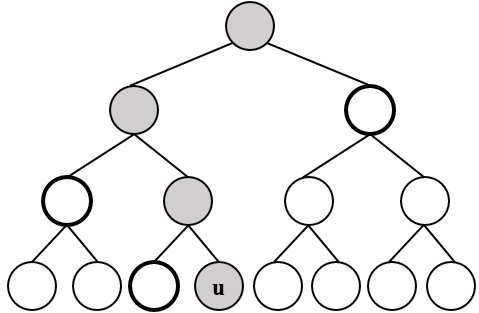
\includegraphics[scale = 0.3]{images/off-path.png}
        \end{figure}
        \vfill
        \begin{center}
          \begin{small}
            Off-path vertices of $u$ are highlighted in bold.
          \end{small}
        \end{center}

      \item[Verification of Contribution]
        The leaf vertex calculates the root label using received off-path labels.
  
        It compares the the calculated label with the received label from the base station.
        
        If those two labels match then it proceeds to the next step with Acknowledgment (ACK) message or with Negative Acknowledgment (NACK) message.

      \item[Collection of Authentication Codes] 
      
        The authentication code for sensor node $A$ with ACK and NACK message is given as follows :
        \begin{equation*}
          \begin{array}{l}
            \mbox{MAC}_{\sk_{A}}( \mbox{N} || \mbox{ACK})\\
            \mbox{MAC}_{\sk_{A}}( \mbox{N} || \mbox{NACK})  
          \end{array}
        \end{equation*}

        After receiving the authentication codes from all of its children it does XOR operation on all the authentication codes including its own authentication code and before sending to its parent.

      \item[Verification of confirmations]
        The base station computes the following:
        \begin{equation*}
          \bigoplus_{i = 1}^n \mbox{MAC}_{\sk_{i}}(\mbox{N} || \mbox{ACK})
        \end{equation*}
        Then it compares the computed code with the received code. 
        If those two codes match, then the base station accepts the aggregation result.

      \end{description}
      \vfill
      \clearpage

\section*{Our Protocol}
    
    \subsection*{Data Item}
      \vfill
      A commitment tree is a binary tree where each vertex has an associated data-item representing the data that is passed on to its parent.
      \begin{equation*}
        < id, count, value, commitment >
      \end{equation*}

      Each sensor node creates its own data-item. 
      For example, sensor node $A$ creates its data-item $A_{0}$.
      \begin{equation*}
        A_{0} =\ <A_{id}, 1, A_{value}, H(N||1||A_{value})>
      \end{equation*}
      where $A_{id}, A_{value}$ is the unique ID and sensor reading of the node $A$. 
      The count is $1$ as there is only vertex in the subtree rooted at $A$, $H$ is the collision resistant hash function, and $N$ is the query nonce.
      \vfill
      \clearpage

    \subsection*{Signing and Verification of the Data-item}
      \vfill
      Each sensor node sends the signature of its data-item signed by itself using its own secret key. 
      \begin{equation*}
          \textsf{S} = \textsf{Sign}_{\sk_{A}}(A_{0})
        \end{equation*}
        \begin{center}
          Table: Digital Certificate
      \end{center}
      \begin{table} 
        \tiny 
          \centering
          \begin{tabular}{ |l| }
              \hline
              Unique ID of the sensor node \\
              \hline
              Public key of the sensor node \\  
              \hline
              Certification Authority's name \\
              \hline
              Certification Authority's digital signature \\
              \hline
          \end{tabular}
        % \end{center}
      \end{table}

      \begin{equation*}
        \textsf{Verify}_{\pk_{A}}(A_{0},\textsf{S}) = 
        \begin{cases}
         \textbf{true}\ \mbox{with probability of 1} & \mbox{if}\ \textsf{S} = \textsf{Sign}_{\sk_{A}}(A_{0})\\
         \textbf{false}\ \mbox{with overwhelming probability} & \mbox{if}\ \textsf{S} \neq \textsf{Sign}_{\sk_{A}}(A_{0})
        \end{cases}
      \end{equation*}
      \vfill
      \clearpage

    \subsection*{Commitment Payload}
      \vfill
      A \textbf{commitment payload} is a set of data-items of the root vertices of the trees with their respective signatures in the outgoing commitment forest and an additional signature for the transmission.
    
      The \textbf{transmit payload} is the concatenation of all the data-items in the commitment payload.
      \vfill
      \clearpage

    \subsection*{Commitment Payload Example}
      \vfill
      \begin{figure}[h!]
        \centering
        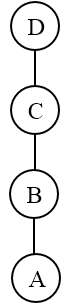
\includegraphics[scale = 0.4]{images/palm-aggregation-tree.png}
        % \caption{Palm Tree}
      \end{figure}
      \begin{center}
        Figure 3: Palm Aggregation Tree
      \end{center}
      \begin{equation*}
        A_{pay} =\ <A_{0}, \textsf{Sign}_{\sk_{A}}(A_{0}), \textsf{Sign}_{\sk_{A}}(A_{\tau}) >\ where\ A_{\tau} =\ < A_{0} > 
      \end{equation*}
      \vfill
      \clearpage

      \vfill
      \begin{figure}
        \centering
        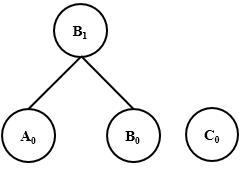
\includegraphics[scale = 0.5]{images/commitment-payload-of-C.png}
        % \caption{Commitment Payload of Sensor Node $C$}
        % \label{fig:Commitment payload of C}
      \end{figure}
      \begin{center}
        Figure 4: Commitment Payload of C
      \end{center}

      \begin{equation*}  
        \begin{array}{l}
          C_{pay} =\ <C_{0},\textsf{Sign}_{\sk_{C}}(C_{0}),B_{1},\textcolor{red}{\textsf{Sign}_{\sk_{B}}(B_{1})}, \textsf{Sign}_{\sk_{C}}(C_{\tau})>\ where\ C_{\tau} = <C_{0} || B_{1}>\\
          C_{0} =\ <C_{id}, 1, C_{value}, H(N||1||C_{value})>\\
          B_{1} =\ <B_{id}, 2, B_{1value}, H(N||2||B_{1value}||A_{0}||B_{0})>;\ B_{1value} =\ B_{value} + A_{value}
        \end{array}
      \end{equation*}
      \vfill
      \clearpage

    \subsection*{FSwRD vs FSwoRD}
      \vfill
      Forwarding Signatures With Resigning Data-Item (FSwRD)
      \begin{equation*}  
        \begin{array}{l}
          C_{pay} =\ <C_{0},\textsf{Sign}_{\sk_{C}}(C_{0}),B_{1},\textcolor{red}{\textsf{Sign}_{\sk_{C}}(B_{1})}, \textsf{Sign}_{\sk_{C}}(C_{\tau})>\ where\ C_{\tau} =\ <C_{0} || B_{1}>\\
        \end{array}
      \end{equation*}

      Forwarding Signatures Without Resigning Data-Item (FSwoRD)
      \begin{equation*}
          C_{pay} =\ <C_{0}, \textsf{Sign}_{\sk_{C}}(C_{0}), B_{1}, \textcolor{red}{\textsf{Sign}_{\sk_{B}}(B_{1})}, \textsf{Sign}_{\sk_{C}}(C_{\tau}) >\ where\ C_{\tau} =\ <C_{0} || B_{1}>\\
      \end{equation*}
      
      \vfill
      \clearpage

    \subsection*{Analogy for FSwRD vs FSwoRD}
      \vfill
      \begin{figure}[h!]
        \centering
        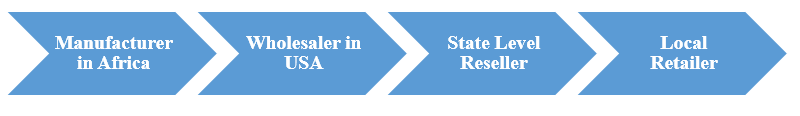
\includegraphics[scale=0.5]{images/diamond-supply-chain.png}
        \caption{Diamond Supply Chain.}
        \label{fig:diamond-supply-chain}
      \end{figure}
      \vfill
      \clearpage

    \subsection*{Security Benefits of Signatures}
      \vfill
      The signature allows the parent node to verify the \textbf{authenticity} of the sensor node and assures the \textbf{integrity} of the data-item.

      It allows the sender to have the proof for the sent data-item and the receiver to have the proof for the received data-item, providing the security service of \textbf{non-repudiation}.

      The digital signature depends on the message so the parent node can not reuse the signature for other messages in the future, protecting the network against the \textbf{replay attacks}.

      The signature of the transmit-payload is like the signature for the transmission, assuring none of the data-items in its payload have been left stranded.

      \vfill
      \clearpage

    \subsection*{Aggregate Commit}
      \vfill
      This phase creates the commitment tree for the given aggregation tree.
      % We describe the commitment tree generation process for an aggregation tree shown in Figure \ref{fig:Aggregation-tree-1}.
      % \begin{figure}[h!]
      %   \centering
      %   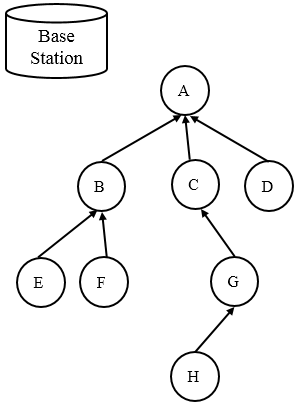
\includegraphics[scale=0.4]{images/aggregation-tree-1.png}
      %   \caption{Aggregation Tree.}
      %   \label{fig:Aggregation-tree-1}
      % \end{figure}

    \subsection*{Commitment Tree Generation}
    
      Leaf nodes in the aggregation tree construct and send their payload to their parents in the aggregation tree.  
      
      Each internal node in the aggregation tree constructs their leaf vertex.
  
      Internal node verifies all the received signatures then it merges all the data-items with same count value from its forest.

      It merges two data-items by creating a new data-item with count value incremented by one and whose value is the addition of value field of the previous two data-items. 

      For example, in Figure \ref{fig:Aggregation-tree-1}, the root $A$ receives payloads from each of its children.
        
      We describe the payload generation process for nodes $D,B,C$ and $A$ in order.
      \vfill
      \clearpage

    \subsection*{Example Continue: D's Payload Generation}
      The node $D$ constructs its payload and sends $D_{pay}$ to its parent $A$.
      
      \begin{figure}[h!]
        \centering
        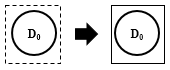
\includegraphics[scale = 0.5]{images/d-forest-payload.png}
        \caption{Transformation from $D$'s forest to its payload.
            Each dashed-line box shows forest and solid-line box shows payload of the respective sensor node.}
        \label{fig:d-forest-payload}
      \end{figure}
      \begin{equation*}
        \begin{array}{l}
          D_{pay} =\ <D_{0}, \textsf{Sign}_{\sk_{D}}(D_{0}), \textsf{Sign}_{\sk_{D}}(D_{\tau})>;\ where\ D_{\tau} =\ <D_{0}>\\
          \\
          D_{0} =\ <D_{id},1,D_{value},H(N||1||D_{value})>
        \end{array}
      \end{equation*}

      \vfill
      \clearpage

    \subsection*{Example Continue: B's Payload Generation}  
      The node $B$ constructs its payload from its forest which consists of payloads received from $E$ and $F$.

      Then node $B$ sends $B_{pay}$ to its parent $A$.
      \begin{figure}[h!]
        \centering
        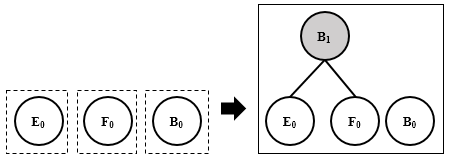
\includegraphics[scale = 0.5]{images/b-forest-payload.png}
        \caption{Transformation from $B$'s forest to its payload.}
        \label{fig:b-forest-payload}
      \end{figure}
      
      % \begin{equation*}
      %   \begin{array}{l}
      %   E_{pay} =\ <E_{0}, \textsf{Sign}_{\sk_{E}}(E_{0}), \textsf{Sign}_{\sk_{E}}(E_{\tau}) >\ where\ E_{\tau} =\ <E_{0}>\\
      %   F_{pay} =\ <F_{0}, \textsf{Sign}_{\sk_{F}}(F_{0}), \textsf{Sign}_{\sk_{F}}(F{\tau}) >\ where\ F_{\tau} =\ <F_{0}>
      %   \end{array}
      % \end{equation*}
      
      \begin{equation*}
        \begin{array}{l}
          B_{1} =\ < B_{id}, 2, B_{1value}, H(N||2||B_{1value}||E_{0}||F_{0})>;\ B_{1value} = E_{value} + F_{value}\\
          \\
          B_{pay} =\ < B_{0}, \textsf{Sign}_{\sk_{B}}(B_{0}), B_{1}, \textsf{Sign}_{\sk_{B}}(B_{1}), \textsf{Sign}_{\sk_{B}}(B_{\tau}) >\ where\ B_{\tau} =\ <B_{0} || B_{1}>\\
        \end{array}
        \label{eq:b-payload}
      \end{equation*}


      \vfill
      \clearpage
    
    \subsection*{Example Continue: C's Payload Generation}  
      The node $C$ constructs its payload from its forest which consists of payloads received from $G$.

      Then node $C$ sends $C_{pay}$ to its parent $A$.

      \begin{figure}[h!]
        \centering
        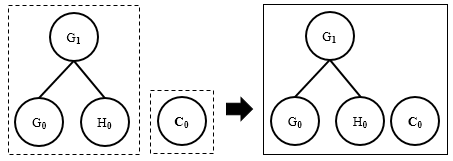
\includegraphics[scale = 0.5]{images/c-forest-payload.png}
        \caption{$C$'s forest aggregation creating its payload.}
        \label{fig:c-forest-payload}
      \end{figure}
      \begin{equation*}
        \begin{array}{l}
          G_{pay} =\ <G_{1},\textcolor{red}{\textsf{Sign}_{\sk_{G}}(G_{1})}, \textsf{Sign}_{\sk_{G}}(G_{\tau})>\ where\ G_{\tau} =\ <G_{0} || H_{0}>\\
        \end{array}
      \end{equation*}
      
      \begin{equation*}
        \begin{array}{l}
          C_{pay} =\ <C_{0},\textsf{Sign}_{\sk_{C}}(C_{0}),G_{1},\textcolor{red}{\textsf{Sign}_{\sk_{C}}(G_{1})}, \textsf{Sign}_{\sk_{C}}(C_{\tau})>\ where\ C_{\tau} =\ <C_{0} || G_{1}>\\
        \end{array}
        %\label{eq:c-payload}
      \end{equation*}

      \vfill
      \clearpage

    \subsection*{Example Continue: A's Payload Generation}  

      The root node of the aggregation tree $A$ receives the payloads from $B,C$ and $D$ respectively.
      
      \begin{figure}[h!]
        \centering
        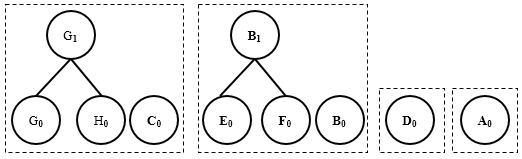
\includegraphics[scale = 0.5]{images/a-forest.png}
        \caption{$A$'s forest: $A$ receives three payloads from $C,B$ and $D$}
        \label{fig:a-forest}
      \end{figure}
      \vfill
      \clearpage

      \begin{figure}[h!]
        \centering
        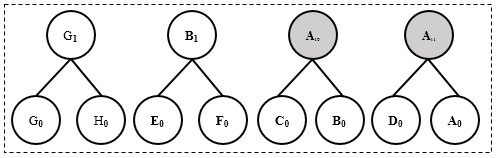
\includegraphics[scale = 0.5]{images/a-forest-first-merge.png}
        \caption{$A$'s forest: after first merge}
        \label{fig:a-forest-first-merge}
      \end{figure}
      \begin{equation*}
        \begin{array}{l}
          A_{10} =\ <A_{id},2,A_{10value},H(N||2||A_{10value}||B_{0}||C_{0})>;\ A_{10value} =\ B_{value} + C_{value}\\
          A_{11} =\ <A_{id},2,A_{11value},H(N||2||A_{11value}||D_{0}||A_{0})>;\ A_{11value} =\ D_{value} + A_{value}\\
        \end{array}     
      \end{equation*}

      \begin{figure}[h!]
        \centering
        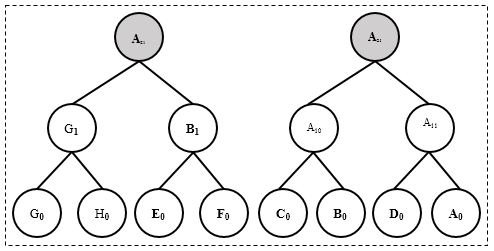
\includegraphics[scale = 0.5]{images/a-forest-second-merge.png}
        \caption{$A$'s forest: after second merge}
        \label{fig:a-forest-second-merge}
      \end{figure}

      \begin{equation*}
        \begin{array}{l}
          A_{20} =\ <A_{id},4,A_{20value},H(N||4||A_{20value}||G_{1}||B_{1})>;\ A_{20value} =\ G_{1value} + B_{1value}\\ 
          A_{21} =\ <A_{id},4,A_{21value},H(N||4||A_{21value}||A_{10}||A_{11})>;\ A_{21value} =\ A_{10value} + A_{11value}\\ 
        \end{array}
      \end{equation*}

      \begin{figure}[h!]
        \centering
        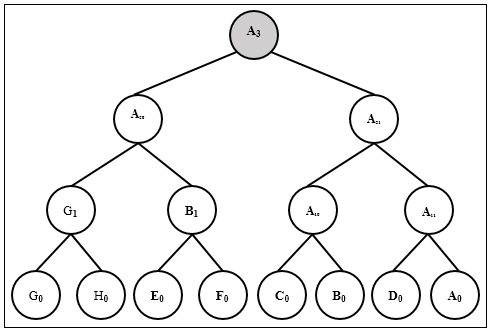
\includegraphics[scale = 0.5]{images/a-payload.png}
        \caption{$A$'s payload : $A$ sends $A_{3}$ to the base station.}
        \label{fig:a-payload}
      \end{figure}

      \begin{equation*}
        \begin{array}{l}
        A_{3} =\ <A_{id}, 8, A_{3value}, H(N||8||A_{3value}||A_{20}||A_{21})>;\ A_{3value} =\ A_{20value} + A_{21value}\\
        A_{pay} =\ <A_{3},\textsf{Sign}_{\sk_{A}}(A_{3}),\textsf{Sign}_{\sk_{A}}(A_{\tau})>\ where\ A_{\tau} =\ <A_{3}>
        \end{array}
      \end{equation*}
     \vfill
     \clearpage

    \subsection*{Result Checking}
      This phase requires that all the sensor nodes verify their individual contributions to the final aggregate value.

      If there is any inconsistency in the aggregation process then with the help of the base station, trace down the node responsible for inconsistency.

      It has the following major steps :
      \begin{description}
        \item [Dissemination of Final Payload by the Base Station]
        \item [Dissemination of Off-Path Values]
        \item [Verification of Inclusion]
        \item [Collection of Authentication Codes]
        \item [Verification of Authentication Codes]
        \item [Detecting An Adversary]
      \end{description}

      \vfill
      \clearpage

    \subsection*{Dissemination of Final Payload by the Base Station}

      The base station broadcasts all the data-items in the payload to entire network using \textbf{authenticated broadcast}.
        
      The base station receives only one data-item $A_{3}$ in the payload sent by $A$.
      
      The base station broadcasts $B_{pay}$ to entire network.

      \begin{equation*}
        \textsf{B}_{pay} =\ <A_{3}, \textsf{Sign}_{\sk_{\textsf{B}}}(A_{3}), \textsf{Sign}_{\sk_{\textsf{B}}}(\textsf{B}_{\tau})>\ where\ \textsf{B}_{\tau} =\ <A_{3}>.
      \end{equation*}
      \vfill
      \clearpage

      \subsection*{Dissemination of Off-Path Values}
        
        In Figure \ref{fig:a-payload}, $A_{10}$ has two children $C_{0}$ and $B_{0}$.
        
        $A_{10}$ also receives $A_{11}$ and $A_{20}$ from its parent $A_{21}$.
        
        $A_{10}$ ( which is sensor node $A$ in aggregation tree ) sends the following off-path values to $C$ and $B$ respectively.
        
        % $A_{10}$ (which is sensor node $A$ in aggregation tree) sends the following off-path values to $C$ and $B$.
        
        % \begin{equation*}
        %   \begin{array}{l}
        %     <B_{0}, \textsf{Sign}_{\sk_{A}}(B_{0}),\textsf{Sign}_{\sk_{A}}(A_{\tau})>\ where\ A_{\tau} =\ <B_{0}>\\
        %     <C_{0}, \textsf{Sign}_{\sk_{A}}(C_{0}),\textsf{Sign}_{\sk_{A}}(A_{\tau})>\ where\ A_{\tau} =\ <C_{0}>.
        %   \end{array}
        % \end{equation*}
        
        \begin{equation*}
          \begin{array}{l}
            <B_{0}, \textcolor{red}{\textsf{Sign}_{\sk_{A}}(B_{0})},A_{11},\textsf{Sign}_{\sk_{A}}(A_{11}),A_{20},\textsf{Sign}_{\sk_{A}}(A_{20}),\textsf{Sign}_{\sk_{A}}(A_{\tau})>\\
              \\
              % \textcolor{white}{XXXXX}where\  A_{\tau} =\ <B_{0}||A_{11}||A_{20}>\\
            <C_{0}, \textcolor{red}{\textsf{Sign}_{\sk_{A}}(C_{0})},A_{11},\textsf{Sign}_{\sk_{A}}(A_{11}),A_{20},\textsf{Sign}_{\sk_{A}}(A_{20}),\textsf{Sign}_{\sk_{A}}(A_{\tau})>\\ 
              % \textcolor{white}{XXXXX}where\  A_{\tau} =\ <C_{0}||A_{11}||A_{20}>.
          \end{array}
        \end{equation*}
        \vfill
        \clearpage

      \subsection*{FSwoRD}
        \begin{equation*}
          \begin{array}{l}
            <B_{0}, \textcolor{red}{\textsf{Sign}_{\sk_{B}}(B_{0})},A_{11},\textsf{Sign}_{\sk_{A}}(A_{11}),A_{20},\textsf{Sign}_{\sk_{A}}(A_{20}),\textsf{Sign}_{\sk_{A}}(A_{\tau})>\\
              \\
              % \textcolor{white}{XXXXX}where\  A_{\tau} =\ <B_{0}||A_{11}||A_{20}>\\
            <C_{0}, \textcolor{red}{\textsf{Sign}_{\sk_{C}}(C_{0})},A_{11},\textsf{Sign}_{\sk_{A}}(A_{11}),A_{20},\textsf{Sign}_{\sk_{A}}(A_{20}),\textsf{Sign}_{\sk_{A}}(A_{\tau})>\\ 
              % \textcolor{white}{XXXXX}where\  A_{\tau} =\ <C_{0}||A_{11}||A_{20}>.
          \end{array}
        \end{equation*}

        In FSwRD, all the leaf vertices need to know only one certificate as they receive data-items signed by their parent vertex.

        In FSwoRD, all the leaf vertices might need to know $\log l$ certificates, where $l$ is the number of leaf-vertices in commitment tree.
        \vfill
        \clearpage

      \subsection*{Significance of Commitment Filed}

        The commitment filed provides data-integrity and helps us detecting any \textit{malicious activity} in the network. 
        The signatures infrastructure eventually we can detect an adversary. 

        If an internal vertex simply \textbf{forwards incorrect data-item} then the relevant leaf vertex will complain, as they will not be able to derive the data-item received using authenticated broadcast from the base station.
        
        If an internal vertex \textbf{changed the data-item} while creating commitment tree and sending the incorrect off-path values to compensate discrepancy. 
        \vfill
        \clearpage

      \subsection*{Malicious Activity}

        Suppose the vertices in the commitment tree have the data-items defined as follows :
        
        \begin{equation*}
          \begin{array}{l}
            A_{0} =\ <A_{id},1,10, H(N||1||10)>\\
            B_{0} =\ <B_{id},1,20, H(N||1||20)>\\
            C_{1} =\ <C_{id},2,30, H(N||2||30||A_{0}||B_{0})>
          \end{array}
        \end{equation*}

        \begin{figure}
          \centering
          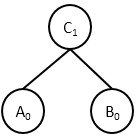
\includegraphics[scale=0.6]{images/commitment-tree-2.png}
          \label{fig:smallest-ct}
          \tiny{\caption{Smallest Possible Commitment Tree}}
        \end{figure}
        \vfill
        \clearpage

        Suppose $C$ changes $A_{0}$ and $B_{0}$ to $A'_{0}$ and $B'_{0}$.

        $C$ can send either $C'_{1}$ or $C''_{1}$ to the base station.
        
        To compensate for the discrepancy, $C$ constructs $B''_{0}$ and $A''_{0}$ off-path values trying to hide its malicious activity from the base station.

        \begin{equation*}
          \begin{array}{l}
            A'_{0} =\ <A_{id},1,100, H(N||1||10)>\\
            B'_{0} =\ <B_{id},1,200, H(N||1||20)>\\
            \\
            C'_{1} =\ <C_{id},2,300, H(N||2||300||\mathbf{A''_{0}}||\mathbf{B_{0}})>\ or \\ 
            C''_{1} =\ <C_{id},2,300, H(N||2||300||\mathbf{A_{0}}||\mathbf{B''_{0}})>\\
            \\
            B''_{0} = <B_{id},1,290,H(N||1||20)>\\
            A''_{0} = <A_{id},1,280,H(N||1||10)>
          \end{array}
        \end{equation*}
        \vfill
        \clearpage

        $A$ and $B$ receives either $C'_{1}$ or $C''_{1}$ from the base station based on what $C$ has sent to base station.

        $A$ and $B$ receives $B''_{0}$ and $A''_{0}$ from $C$ respectively.

        $A$ and $B$ derives the root data-item using the received off-path values, and it does not match with the received root data-item.

        \begin{equation*}
          \begin{array}{l}
            A\ \mbox{uses}\ (A_{0}, B''_{0})\ \mbox{and derives} <2,300,H(N||2||300||\mathbf{A_{0}}||\mathbf{B''_{0}})>\  = C''_{1} \neq C'_{1} \\
            B\ \mbox{uses}\ (A''_{0}, B_{0})\ \mbox{and derives} <2,300,H(N||2||300||\mathbf{A''_{0}}||\mathbf{B_{0}})>\  = C'_{1} \neq C''_{1}.
          \end{array}
        \end{equation*}

        The commitment field makes it nearly impossible for an adversary to tamper with the data-items while creating commitment tree and/or while distributing off-path values.
        \vfill
        \clearpage

      \subsection*{Verification of Inclusion}
        \vfill
        Sensor node verifies that no aggregation tampering has occurred on the path between its leaf vertex and the root of its commitment tree.

        It is able to do so since the off-path values provide all the necessary information to perform the data-item computation.

        In the previous example, $C$ receives $B_{0}, A_{11}$ and $ A_{20}$ from its parent node and it has $C_{0}$.
 
        Then it compares the derived $A_{3}$ with the $A_{3}$ received from the base station.

        If those data-items are identical then the node sends the authentication code with ACK message and if those data-items are not identical then the node sends the authentication code with NACK message.
        \vfill
        \clearpage

      \subsection*{Collection of Authentication codes}
        \vfill
        For sensor node $I$ authentication codes are given as follows:
        \begin{equation}
          \begin{array}{l}
            \mbox{Positive : } \mbox{MAC}_{\sk_{I}}(\mbox{N} || \mbox{ACK})\\
            \mbox{Negative : } \mbox{MAC}_{\sk_{I}}(\mbox{N} || \mbox{NACK})
          \end{array}
        \end{equation}        
        $\sk_{I}$ is the secret key of the sensor node $I$, ACK and NACK are special messages.

        An internal sensor node computes the XOR of its own authentication code with all the received codes, and forwards it to its parent.
 
        For example, the sensor node $B$, sends the following authentication code to $A$.
        \begin{equation*}
          \mbox{MAC}_{\sk_{E}}(\mbox{N}||\mbox{ACK}) \oplus \mbox{MAC}_{\sk_{F}}(\mbox{N}||\mbox{ACK}) \oplus \mbox{MAC}_{\sk_{B}}(\mbox{N}||\mbox{ACK})
        \end{equation*}
        \vfill
        \clearpage

      \subsection*{Verification of Authentication codes}
        \vfill
        The base station computes the $\Delta_{ack}$ as follows :
        \begin{equation*}
          \displaystyle{\Delta_{ack} = \bigoplus_{i = 1}^n \mbox{MAC}_{\sk_{i}}(\mbox{N} || \mbox{ACK}) }
        \end{equation*}
        Here, the addition represents an XOR operation.

        The base station compares   $\Delta_{ack}$ with the received root authentication code $\Delta_{root}$. 
        
        If those two codes match then it accepts the aggregated value or else it proceeds further to find an adversary. 

        The base station identifies the nodes who sent their authentication codes with NACK called a complainer. 
        
        The base station can find a single complainer complainer in \textbf{linear time}.

        \vfill
        \clearpage

      \subsection*{Identifying more than one complainer}
        \vfill
        
        \begin{algorithm}
          \caption{Finding complainer tree in a given forest}
          \label{algo:detect-a-complainer-tree}
          \begin{algorithmic}[1]
            \STATE BS requests authentication codes of all the tree roots in the aggregation tree root's forest.
            \STATE BS simulates authentication codes of all the tree roots in the aggregation tree root's forest with ACK message.
            \STATE BS compares the requested and simulated authentication codes.
            \STATE BS constructs \textsf{T} = $\{\textsf{T}_{1},\textsf{T}_{2},\dotsc,\textsf{T}_{n}\}$ whose authentication codes do not match.
            \FORALL {$t \in \textsf{T}$}
              \STATE Call Algorithm \ref{algo:detect-a-complainer} with ($t$)     
            \ENDFOR 
          \end{algorithmic}
        \end{algorithm}

        \begin{algorithm}
          \caption{Finding complainer node in a given tree}
          \label{algo:detect-a-complainer}
          \begin{algorithmic}[1]
            \STATE BS requests the authentication codes of child $C_{1}$ and $C_{2}$ for the given tree.
            \STATE BS simulates the authentication codes of child $C_{1}$ and $C_{2}$ with ACK message.
            \STATE BS compares the requested and simulated authentication codes and identifies $C'$ whose authentication codes do not match.
            \IF {$C'$ is a leaf vertex}
              \STATE Add $C'$ to complainer vertex set \sf{C} 
            \ELSE
              \STATE Call Algorithm \ref{algo:detect-a-complainer} with ($C'$)      
            \ENDIF
          \end{algorithmic}
        \end{algorithm}

        % Note the fact that, in Algorithm \ref{algo:detect-a-complainer}, one of the child nodes will not match with the simulated authentication codes of the base station.
        % These algorithms are recursive and runs in exponentially time.
        % This algorithm detects complainers faster if there are more complainers in the same commitment tree.
        % Hence, we expect this algorithm to run in linear time.

        \vfill
        \clearpage

      \subsection*{Detecting an Adversary}
        \vfill
    
        Based on the complainer set $\textsf{C}$ it constructs a set of possible adversaries $\textsf{A} = \{\textsf{A}_{1},\textsf{A}_{2},\dotsc,\textsf{A}_{n}\}$. 

        \begin{figure}[t]
          \centering
          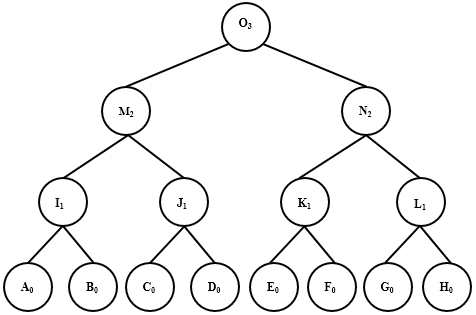
\includegraphics[scale=0.4]{images/possible-cheaters.png}
          % \label{fig:cheating}
        \end{figure}

        Suppose $\textsf{C}=\{A_{0}\}$ then $\textsf{A} =\{I,\{B,I\},\{B,M\},\{B,I,M\}\}$. 

        Note the fact that only $I$ knows the exact data-item of $A_{0}$. 
        
        The vertices $M$ and $O$ knows aggregated value of $A_{0}$. 
        
        Hence, if either $M$ or $O$ tampers they tamper with more than one data-item or they have to cheat in a group. 

      \subsection*{Detecting a single adversary}
        \vfill
        Suppose, $I$ is an adversary and $\textsf{C} = \{A_{0}\}$ then $\textsf{A}=\{I,\{B,I\},\{B,M\},\{B,I,M\}\}$.
        \begin{equation*}
          \begin{array}{l}
            I_{1} =\ <I_{id}, 1, I_{1value}, H(N||1||I_{value}||\mathbf{A_{0}}||B_{0})> \\ 
            I_{pay} =\ <I_{1}, \textsf{Sign}_{\sk_{I}}(I_{1}), \textsf{Sign}_{\sk_{I}}(I_{\tau})>\\
          \end{array}
        \end{equation*}
        Whereas,
        \begin{equation*}
          \begin{array}{l}
            I'_{1} =\ <I_{id}, 1, I'_{1value}, H(N||1||I'_{value}||\mathbf{A'_{0}}||B_{0})> \\
            I'_{pay} =\ <I'_{1}, \textsf{Sign}_{\sk_{I}}(I'_{1}), \textsf{Sign}_{\sk_{I}}(I_{\tau})> \mbox{where}\ I_{\tau} = I'_{1}.\\
          \end{array}
        \end{equation*}
        First the base station asks $A$ to send its payload.
        \begin{equation*}
          \begin{array}{l}
          A_{pay} =\ <A_{0}, \textsf{Sign}_{\sk_{A}}(A_{0}), \textsf{Sign}_{\sk_{A}}(A_{\tau})>\\
          A_{0} =\ <A_{id}, 1, A_{value}, H(N||1||A_{value})>
          \end{array}
        \end{equation*}

        The base station asks $I$ to send its own payload.
        $I$ sends its false payload to the base station.
        \begin{equation*}
          \begin{array}{l}
            A_{pay} = <A_{0}, \textsf{Sign}_{\sk_{A}}(A_{0}), \textsf{Sign}_{\sk_{A}}(A_{\tau})> \mbox{where}\ A_{\tau} = A_{0}\\
            B_{pay} = <B_{0}, \textsf{Sign}_{\sk_{B}}(B_{0}), \textsf{Sign}_{\sk_{A}}(B_{\tau})> \mbox{where}\ B_{\tau} = B_{0}\\
            I_{pay} = <I_{1}, \textsf{Sign}_{\sk_{I}}(I_{1}), \textsf{Sign}_{\sk_{A}}(I_{\tau})> \mbox{where}\ I_{\tau} = I_{0}\\
          \end{array}
        \end{equation*}
        Then the base station asks $M$ to send all the received payload from each of its children.
        \begin{equation*}
          \begin{array}{l}
            I'_{pay} = <I'_{1}, \textsf{Sign}_{\sk_{I}}(I'_{1}), \textsf{Sign}_{\sk_{I}}(I_{\tau})> \mbox{where}\ I_{\tau} = I'_{1}\\
            J_{pay} = <J_{1}, \textsf{Sign}_{\sk_{I}}(J_{1}), \textsf{Sign}_{\sk_{A}}(J_{\tau})> \mbox{where}\ J_{\tau} = J_{0}\\
          \end{array}
        \end{equation*}
        As the base station receives the $I'_{pay}$ with a signature from $M$, it proves that $I$ is an adversary.
        \vfill
        \clearpage

      \subsection*{Algorithm to Detect an Adversary}
        \begin{algorithm}
          \caption{Pseudo algorithm to detect an adversary}
          \label{algo:detect-an-adversary}
          \begin{algorithmic}[1]

            \STATE BS\ identifies all the complainer and constructs $\textsf{C} = \{\textsf{C}_{1}, \textsf{C}_{2}, \dotsc, c\textsf{C}_{n}\}$
            \FORALL {$C \in \textsf{C}$}

              \STATE BS asks $C$ to send data-item with its signature, sent during commitment tree generation phase
            
            \ENDFOR

            \STATE BS identifies possible adversary based on $\textsf{C}$ and constructs $\textsf{A} = \{\textsf{A}_{1},\textsf{A}_{2},\dotsc,\textsf{A}_{n}\}$

            \FORALL {$A \in \textsf{A}$}

              \STATE BS asks $A$ to send data-items with its signature, received and sent by $A$ during commitment tree generation phase
              \STATE If needed BS  asks the parent of $A$ to send data-items with its signature
        
            \ENDFOR

            \STATE BS determines the adversary based on the verification of signatures

          \end{algorithmic}
        \end{algorithm}

        Once the base station detects adversaries it dispels them from the network for all the future queries.

        Doing so removes un-necessary communication for debugging purpose in the future which saves bandwidth and increases the life-time of the network.        
        \vfill
        \clearpage

      \subsection*{Binary Tree is optimal}
        % \vfill
        \begin{theorem}
          Binary commitment tree is optimal in terms of verification for $m$-ary tree, as it requires minimum number of off-path values.
        \end{theorem}
        \begin{proof}
          Consider the case of a tertiary tree, other $m$-ary tree arguments follows the same manner.
          Let $m$ be the number of leaves in a commitment tree.
          
          For the given binary commitment tree, each leaf vertex needs $\log_2 m$\ off-path values in the verification phase.
          The total off-path values needed in the given commitment tree is [${m \log_2 m}$].
          For the given tertiary commitment tree, each leaf vertex needs $2 \log_3 m$ off-path values in the verification phase.
          The total off-path values needed in given commitment tree is [$2 m \log_3 m$].
            \begin{equation*}
              \begin{array}{l}
                \mbox{Let}\  y = \log_3 m\\
                y = \frac{ {\log _2 m } }{{\log _2  3 }}\ \mbox{where}\ \log_2 3 > 1\\
                y \log_2 3 = \log _2 m \\
                \log_3 m \cdot \log_2 3 = \log _2 m \\
                \log_3 m = \frac{ {\log _2 m } }{{\log _2  3 }} \\
                2m\log_3 m = 2m\frac{ {\log _2 m } }{{\log _2  3 }} = \frac{ {2 } } {{\log _2  3 }}m\log _2 m \\
                2m\log_3 m = (1.2618)m\log _2 m \\
                2m\log_3 m > m\log _2 m \\

              \end{array}
            \end{equation*}
          Hence, in totality the binary commitment tree requires the minimum number of off-path values.
        \end{proof}        
        \vfill
        \clearpage

      \subsection*{Analysis}
        \vfill
        For an aggregation tree with $n$ nodes, at max there will be $\mathbf{(2^{\lg n + 1} - 1) = (2n-1)}$ vertices in the commitment tree.

        In FSwRD and FSwoRD, there are at least $\mathbf{2(2n-1)}$ signatures created while creating the commitment tree.

        In general, an intermediate node with $n$ descendants receives $\mathbf{\lceil \log_2 n \rceil}$ trees from its children.
        
        The node with $n$ descendants receives at least $\mathbf{2 \lceil \log_2 n \rceil} $ signatures.

        We claim that the binary representation of a non-negative number $x$ illustrates the payload decomposition of the sensor node $S$, where $x$ = $1$ + number of descendants of $S$.

        Suppose, sensor node $S$ has $22$ descendants then $x =23$, $(x)_{10}$ = $(10111)_{2}$. 
        This means $S$ has four complete binary trees in its payload, with the height of four, two, one and zero.
        \vfill
        \clearpage
      \subsection*{Analysis}
        \vfill
        \begin{tiny}
          \begin{table}
            \begin{center}
              \begin{tabular}{|c||c|}
                \hline
                Network Topology & Totality of Signatures Transmitted \\ 
                \cline{2-2}
                 & FSwRD \mbox{   } \vline \mbox{   } FSwoRD \\
                \hline
                \hline
                Star & $2n$ \vline \mbox{   }$2n$ \\
                \hline
                Palm Tree & $2n$ \vline \mbox{   }$2n$\\
                \hline
                Complete Binary & $2n$ \vline \mbox{   }$2n$\\
                \hline
              \end{tabular}
            \end{center}
          \end{table}

           \begin{table}
            \begin{center}
              \begin{tabular}{|c||c|}
                \hline
                Network Topology & Totality of Certificates \\ 
                \cline{2-2}
                 & FSwRD \mbox{   } \vline \mbox{   } FSwoRD \\
                \hline
                \hline
                Star & $n - 1$ \vline \mbox{   }$n -1$ \\
                \hline
                Palm Tree & $XX$ \vline \mbox{   }$n - 1$\\
                \hline
                Complete Binary & $n - 1$ \vline \mbox{   }$n - 1$\\
                \hline
              \end{tabular}
            \end{center}
          \end{table}
        \end{tiny}
        \vfill
        \clearpage 
    \subsection*{Conclusion And Future Work}
      \vfill
      Improved SHIA by removing the redundant field in its data-item.
      
      An efficient mathematical way of analyzing the protocol. 
      
      An algorithm to find all possible cheater in the network.
      
      An algorithm which can detect an adversary in the network and remove it for all future queries.
      
      The proof that complete binary tree is an optimal data structure to build the commitment tree.

      In the future, we would like to analyze this protocol for various network topologies and generalized the results.

      It is our hope that further research can improve the cheater detection algorithm.

      \vfill
      \clearpage
      \vfill
        \begin{center}
          \Huge 
          Thank You.  

          Questions ?
        \end{center}
      \clearpage

\end{slide}
\end{document}